\documentclass[10pt,a4paper]{article}
\usepackage[utf8]{inputenc}
\usepackage[T1]{fontenc}
\usepackage[english]{babel}
\usepackage[gen]{eurosym}
\usepackage[table]{xcolor}
\usepackage{graphicx}
\usepackage{wrapfig}
\usepackage[hyphens]{url}
\usepackage[hidelinks]{hyperref}
\usepackage{newcent}
\usepackage{color}
\usepackage{pdfpages}
\usepackage{subfig}

\makeatletter
\author{Stefan Derkits \\
Waldgasse 22/4 \\
1100 Vienna \\
Austria \\
Email: stefan@derkits.at \\
Cell phone: +43 650 602 57 19} \let\Author\@author
\hyphenation{A-ka-de-my}

\title{Akademy 2014 Proposal}

\renewcommand{\familydefault}{\sfdefault}

\definecolor{kdelight}{RGB}{68,104,136}
\definecolor{kdedarker}{RGB}{35,94,154}
\renewcommand\section{%
\@startsection{section}{1}{\z@}%
              {-3.5ex \@plus -1ex \@minus -.2ex}%
              {2.3ex \@plus.2ex}%
              {\color{kdelight}\sffamily\LARGE\bfseries}}
\renewcommand\subsection{%
\@startsection{subsection}{2}{\z@}%
              {-3.25ex\@plus -1ex \@minus -.2ex}%
              {1.5ex \@plus .2ex}%
              {\color{kdelight}\sffamily\Large\bfseries}}
\renewcommand\subsubsection{%
\@startsection{subsubsection}{2}{\z@}%
              {-3.25ex\@plus -1ex \@minus -.2ex}%
              {1.5ex \@plus .2ex}%
              {\color{kdedarker}\sffamily\large\bfseries}}

\let\stdl@section\l@section
\renewcommand*{\l@section}[2]{%
  \stdl@section{\textcolor{kdelight}{#1}}{\textcolor{kdelight}{#2}}}
\let\stdl@subsection\l@subsection
\renewcommand*{\l@subsection}[2]{%
  \stdl@subsection{\textcolor{kdelight}{#1}}{\textcolor{kdelight}{#2}}}
  \let\stdl@subsubsection\l@subsubsection
\renewcommand*{\l@subsubsection}[2]{%
  \stdl@subsubsection{\textcolor{kdelight}{#1}}{\textcolor{kdelight}{#2}}}

\begin{document}

\pagenumbering{gobble}

% \includepdf{proposal-title.pdf}
 
\clearpage
\pagenumbering{arabic}

\tableofcontents
\cleardoublepage

\section*{Summary}
\addcontentsline{toc}{section}{Summary}
Reading the Call for Hosts for Akademy 2018 was great, published a long time before the conference should happen.
In informal talks, we found together as organizers and started to gather ideas and worked on creating this proposal for organizing Akademy 2018 in Vienna.

\subsection*{Community}
\addcontentsline{toc}{subsection}{Community}
The Austrian KDE community is still very small compared to many other cities. At the Akademy 2014 in Brno, we had a KDE Austria BoF and created the kde-at Mailinglist.
Since then we've met up a few times and now want to organize Akademy 2018. We believe Vienna can get together a big number of KDE supporters from all over the world
due to it's central location in the heart of Europe. Also due to the proposed venue at the Technical University of Vienna, Akademy can reach over 5000 talented computer science students.

\subsection*{Date}
\addcontentsline{toc}{subsection}{Date}
Since the proposed venue is a university campus, Akademy should take
place during the summer break which starts at the beginning of July and
ends at the end of September.

\subsection*{Local Support}
\addcontentsline{toc}{subsection}{Local Support}
KDE has many supporters and contributors in Central and Eastern \mbox{Europe}.
Akademy 2018 in Viena will be a great opportunity
for KDE to grow the community even more.

Brno has a strong and lively
Free Software community. Many talented students who are interested in
Linux technologies might get interested in KDE and our software. The
university, where the conference will take place, has several research
projects in the field of computer graphics and desktop. Also the very
active Openmobility group which associates people interested in open
mobile technologies operates from here. Brno's Linux community is
organized in the "Linux in Brno" group that supports the idea of
\mbox{Akademy} in Brno.

\newpage

\subsection*{Local Organizations that Support our Candidacy}
\addcontentsline{toc}{subsection}{Local Organizations that Support out Candidacy}
\begin{description}
\item[\color{kdedarker} AbcLinuxu.cz] -- one of the biggest Czech portals about Linux
\item[\color{kdedarker} Fedora.cz] -- a non-profit organization which is run by the Czech Fedora community and organizes workshops, release parties etc.
\item[\color{kdedarker} Linux in Brno] -- a local Linux user group which organizes meetings, workshops, conferences etc.
\item[\color{kdedarker} Openmobility] -- a non-profit organization that associates open mobile technology enthusiasts and organizes Openmobility conference.
\item[\color{kdedarker} Student Union of FIT] -- organizes many student events, runs several courses and labs and participates in organizing conferences such as \mbox{LinuxAlt}.

\end{description}

\subsection*{Organizers}
\addcontentsline{toc}{subsection}{Organizers}
\begin{description}
\item[\color{kdedarker} KDE Community] -- the KDE community is strong in the Czech Republic and all of the organizers are part of it.
\item[\color{kdedarker} Faculty of Information Technology] -- Brno University of Technology (FIT BUT) -- one of the biggest and most influential IT universities in the Czech Republic -- \url{http://www.fit.vutbr.cz}
\end{description}

\newpage

\subsection*{Organizing Team}
\addcontentsline{toc}{subsection}{Organizing Team}
People from Vienna who have been working on the proposal
and expressed their willingness to help organize the conference.

\subsubsection*{Stefan Derkits}

\subsubsection*{Joseph Wenninger}

\subsubsection*{??Jan Vales??}



\subsubsection*{Elisabeth Hafner}


\vspace{10pt}
\noindent More people have already promised to help in later phases of organizing.

\subsection*{Previously organized events}
\addcontentsline{toc}{subsection}{Previously organized events}
In the past we already organized events ranging from around 5 up to 200 people. Not all of them were FOSS or IT related, but netherless show our organizing skills.

\begin{description}
\item[\color{kdedarker} KDE Austria Meetups] -- Irregular meetups of the KDE community in Vienna
\item[\color{kdedarker} KIF - Konferenz der Informatik Fachschaften] -- Around new years eve 2012 Fachschaft Informatik invited over 50 people from other Universities for a 5 day get-together to Vienna
\item[\color{kdedarker} CouchSurfing Vienna Calling] -- 5 day meetup of around 200 international travellers including BBQs, Parties and other activities
\item[\color{kdedarker} CouchSurfing Vienna Stammtisch] -- monthly CouchSurfing meetup in Vienna, every month a different location, with up to 100 people
\end{description}

\cleardoublepage

\section*{Budget}
\addcontentsline{toc}{section}{Budget}
The budget is based on information we have so far collected and on additional careful estimations. TODO: correct values

\begin{center}
\newcolumntype{L}[1]{>{\raggedright\let\newline\\\arraybackslash\hspace{0pt}}m{#1}}
\begin{tabular}{|L{4cm}|r|r|}
\hline
& \multicolumn{2}{c|}{Alternatives} \\ \hline
& Low & High \\ \hline

Venue & \euro{6,479} & \euro{6,497} \\ \hline
\hspace{20pt}Rent & \euro{4,455} & \euro{4,455} \\ \hline
\hspace{20pt}Energies & \euro{604} & \euro{604}  \\ \hline
\hspace{20pt}Technician \footnotesize{\euro{17}/hr.} & \euro{1,046} & \euro{1,046} \\ \hline
\hspace{20pt}Cleaning & \euro{374} & \euro{374} \\ \hline

Catering & \euro{2,860} & \euro{6,690} \\ \hline
\hspace{20pt}School Cantina

\hspace{20pt}\footnotesize{(Sat-Thu)} & \euro{2,550} & \euro{2,550} \\ \hline
\hspace{20pt}Lunch Meals & \euro{0} & \euro{3,830} \\ \hline
\hspace{20pt}Coffee Breaks & \euro{310} & \euro{310} \\ \hline

SWAG & \euro{1.500} & \euro{2,500} \\ \hline

Social Events & \euro{1,820} & \euro{4,030} \\ \hline
\hspace{20pt}Venue Rent & \euro{1,250} & \euro{1,250} \\ \hline
\hspace{20pt}DJ & \euro{280} & \euro{280} \\ \hline
\hspace{20pt}Drinks and Meals & \euro{290} & \euro{2,500} \\ \hline \hline

Total & \euro{12,659} & \euro{19,717} \\
\hline
\end{tabular}
\end{center}

\cleardoublepage

\section*{Vienna}
\addcontentsline{toc}{section}{Vienna}
\subsection*{The City}
\addcontentsline{toc}{subsection}{The City}
\begin{wrapfigure}{r}{0.5\textwidth}
\vspace{-22pt}
\begin{center}
\includegraphics[width=60mm]{vienna_karlsplatz.jpg}
\footnotesize{Source: Wikipedia}
\end{center}
\vspace{-20pt}
\end{wrapfigure}
Vienna (Wien) is the capital city of Austria. It is in the east of the country on the river Danube. More than 1,800,000 people live there (2016). It is the largest city in Austria. It is also an administrative district (Bundesland) of its own.\\
Before World War I, it was the capital of the Austro-Hungarian Empire. Its centre is a UNESCO World Heritage Site.\\
{\footnotesize{Source: Wikipedia}}\\
\\
For the 8th year in a row, Vienna is ranked number one city according to the Mercer quality of living survey. For a city with nearly 2 million inhabitants, Vienna is a very safe city. The 2017 Global Peace Index ranks Vienna at the 4th place.

\subsection*{Places of Interest}
\addcontentsline{toc}{subsection}{Places of Interest}

\begin{description}
\item[\color{kdedarker} Špilberk Castle] The famous fortress oversees the the city. Currently, \mbox{Špilberk} houses a museum with restaurant.
\item[\color{kdedarker} Petrov Cathedral] St. Peter and Paul Cathedral, known as Petrov forms a dominant silhouette of Brno skyline.
\item[\color{kdedarker} Old Town Hall] See the beloved Brno symbols: the Dragon (Brněnský drak) and the Wheel. The Lopsided tower throwns the entrance. Legend has it that the city council cheated the builder and the tower was his way of payback.
\item[\color{kdedarker} Tugendhat Villa] The villa is listed on the UNESCO World Heritage List. Designed by Mies van der Rohe, it is seen to be a classic example of Bauhaus architecture, and was also the location of the meeting which decided upon the Velvet Divorce that separated the Czech Republic and Slovakia in 1992.
\item[\color{kdedarker} Capuchin Monastery] The 17th century monastery lies right in the city center. Visitors are astonished by its beautiful Baroque statues and mummified monks in the underground tombs.
\item[\color{kdedarker} The Mendel Museum of Genetics] The most famous biologist in the history of genetics worked and died in Brno. This interesting museum commemorates his revolutionary research.
\item[\color{kdedarker} Museum of Roma Culture] The only museum in Central Europe dedicated to the Roma culture.
\end{description}

\begin{flushright}Wikitravel\end{flushright}


\begin{figure}[ht]
\begin{center}
% \includegraphics[width=\textwidth]{spilberk.jpg}
\footnotesize{Špilberk Castle | Source: Marcel Musil (CC-BY-SA)}
\end{center}
\end{figure}

\begin{flushright}Wikitravel \& Wikipedia\end{flushright}

\subsection*{Local IT Industry}
\addcontentsline{toc}{subsection}{Local IT Industry}
Brno has become the Silicon Valley of Central Europe. Several
universities have large ICT faculties that cater to Brno's need for IT
expert. The significant presence of IT firms and R\&D centers attract
professionals from abroad who add to the city's cosmopolitan
atmosphere. A~list of the most important IT companies in Brno:

\begin{description}
\item[\color{kdedarker} 2K Czech] (formerly Illusion Softworks) -- the producer of world-famous PC game titles such as Mafia, Mafia II, Vietcong, Hidden \& Dangerous was founded and has about 200 employees in Brno.
\item[\color{kdedarker} Accenture] -- has a delivery center with about 500 IT professionals.
\item[\color{kdedarker} AVG Technologies] -- the company, which produces the world-known antivirus and security software, was founded and has its headquarters and a large development and research center in Brno.
\item[\color{kdedarker} CZ.NIC] -- is an association that serves as a cz domain registry. It largely supports open source and develops several open-source projects. CZ.NIC's research lab is located in Brno.
\item[\color{kdedarker} IBM] -- opened Global Services Delivery Center 10 years ago. It employs about 2,500 IT professionals in Brno nowadays.
\item[\color{kdedarker} IBA] -- one of the biggest providers of IT services in Central and Eastern Europe has a development center in Brno.
\item[\color{kdedarker} Honeywell] -- the company, which produces a variety of consumer products, engineering services, and aerospace systems, has a large development center with over 700 engineers in Brno.
\item[\color{kdedarker} NetSuite] -- recently opened its development center with 200 engineers in Brno.
\item[\color{kdedarker} Red Hat] -- has its biggest development office in Brno, over 600 engineers work on many opensource projects including the Linux desktop.
\item[\color{kdedarker} Seznam.cz] -- is the biggest Czech Internet company and one of the last few companies whose search engines are more popular than Google in their local markets. It has about 100 developers in Brno.
\item[\color{kdedarker} Siemens] -- Siemens' subsidiary ANF Data has a large development center with around 200 engineers in Brno.
\item[\color{kdedarker} Solar Winds] -- a leader in downloadable network management software has a development center in Brno.
\item[\color{kdedarker} Y Soft] -- is a Brno-based, globally operating company that provides print system management solutions.
\item[\color{kdedarker} ZONER software] -- is a Brno-based software company which is known for its desktop products -- Zoner Draw and Zoner Photo Studio.
\item And many more smaller IT companies.
\end{description}

\subsection*{Local Press}
\addcontentsline{toc}{subsection}{Local Press}
Some Austrian newspapers have dedicated IT news sections or online portals. The most popular are:

\begin{itemize}
\item WebStandard \url{https://derstandard.at/Web}
\item futurezone \url{https://futurezone.at/}
\item Computerwelt \url{http://www.computerwelt.at/}
\end{itemize}


\subsection*{Other community organized IT conferences in Vienna}
\addcontentsline{toc}{subsection}{Other community organized IT conferences in Vienna}
Vienna is the host city for a few regular IT conferences. These include:

\begin{itemize}
	\item LinuxWochen Wien (focused on diverse FOSS topics)
	\item DevFest Vienna (mixed topics)
	\item BSides Vienna (focused on information security)
\end{itemize}

Another upcoming FOSS conference in Vienna is DrupalCon Vienna 2017, happening in September this year.

\subsection*{How to Get to Vienna}
\addcontentsline{toc}{subsection}{How to Get to Vienna}
\subsubsection*{By Plane}
V

\begin{figure}[ht]
\begin{center}
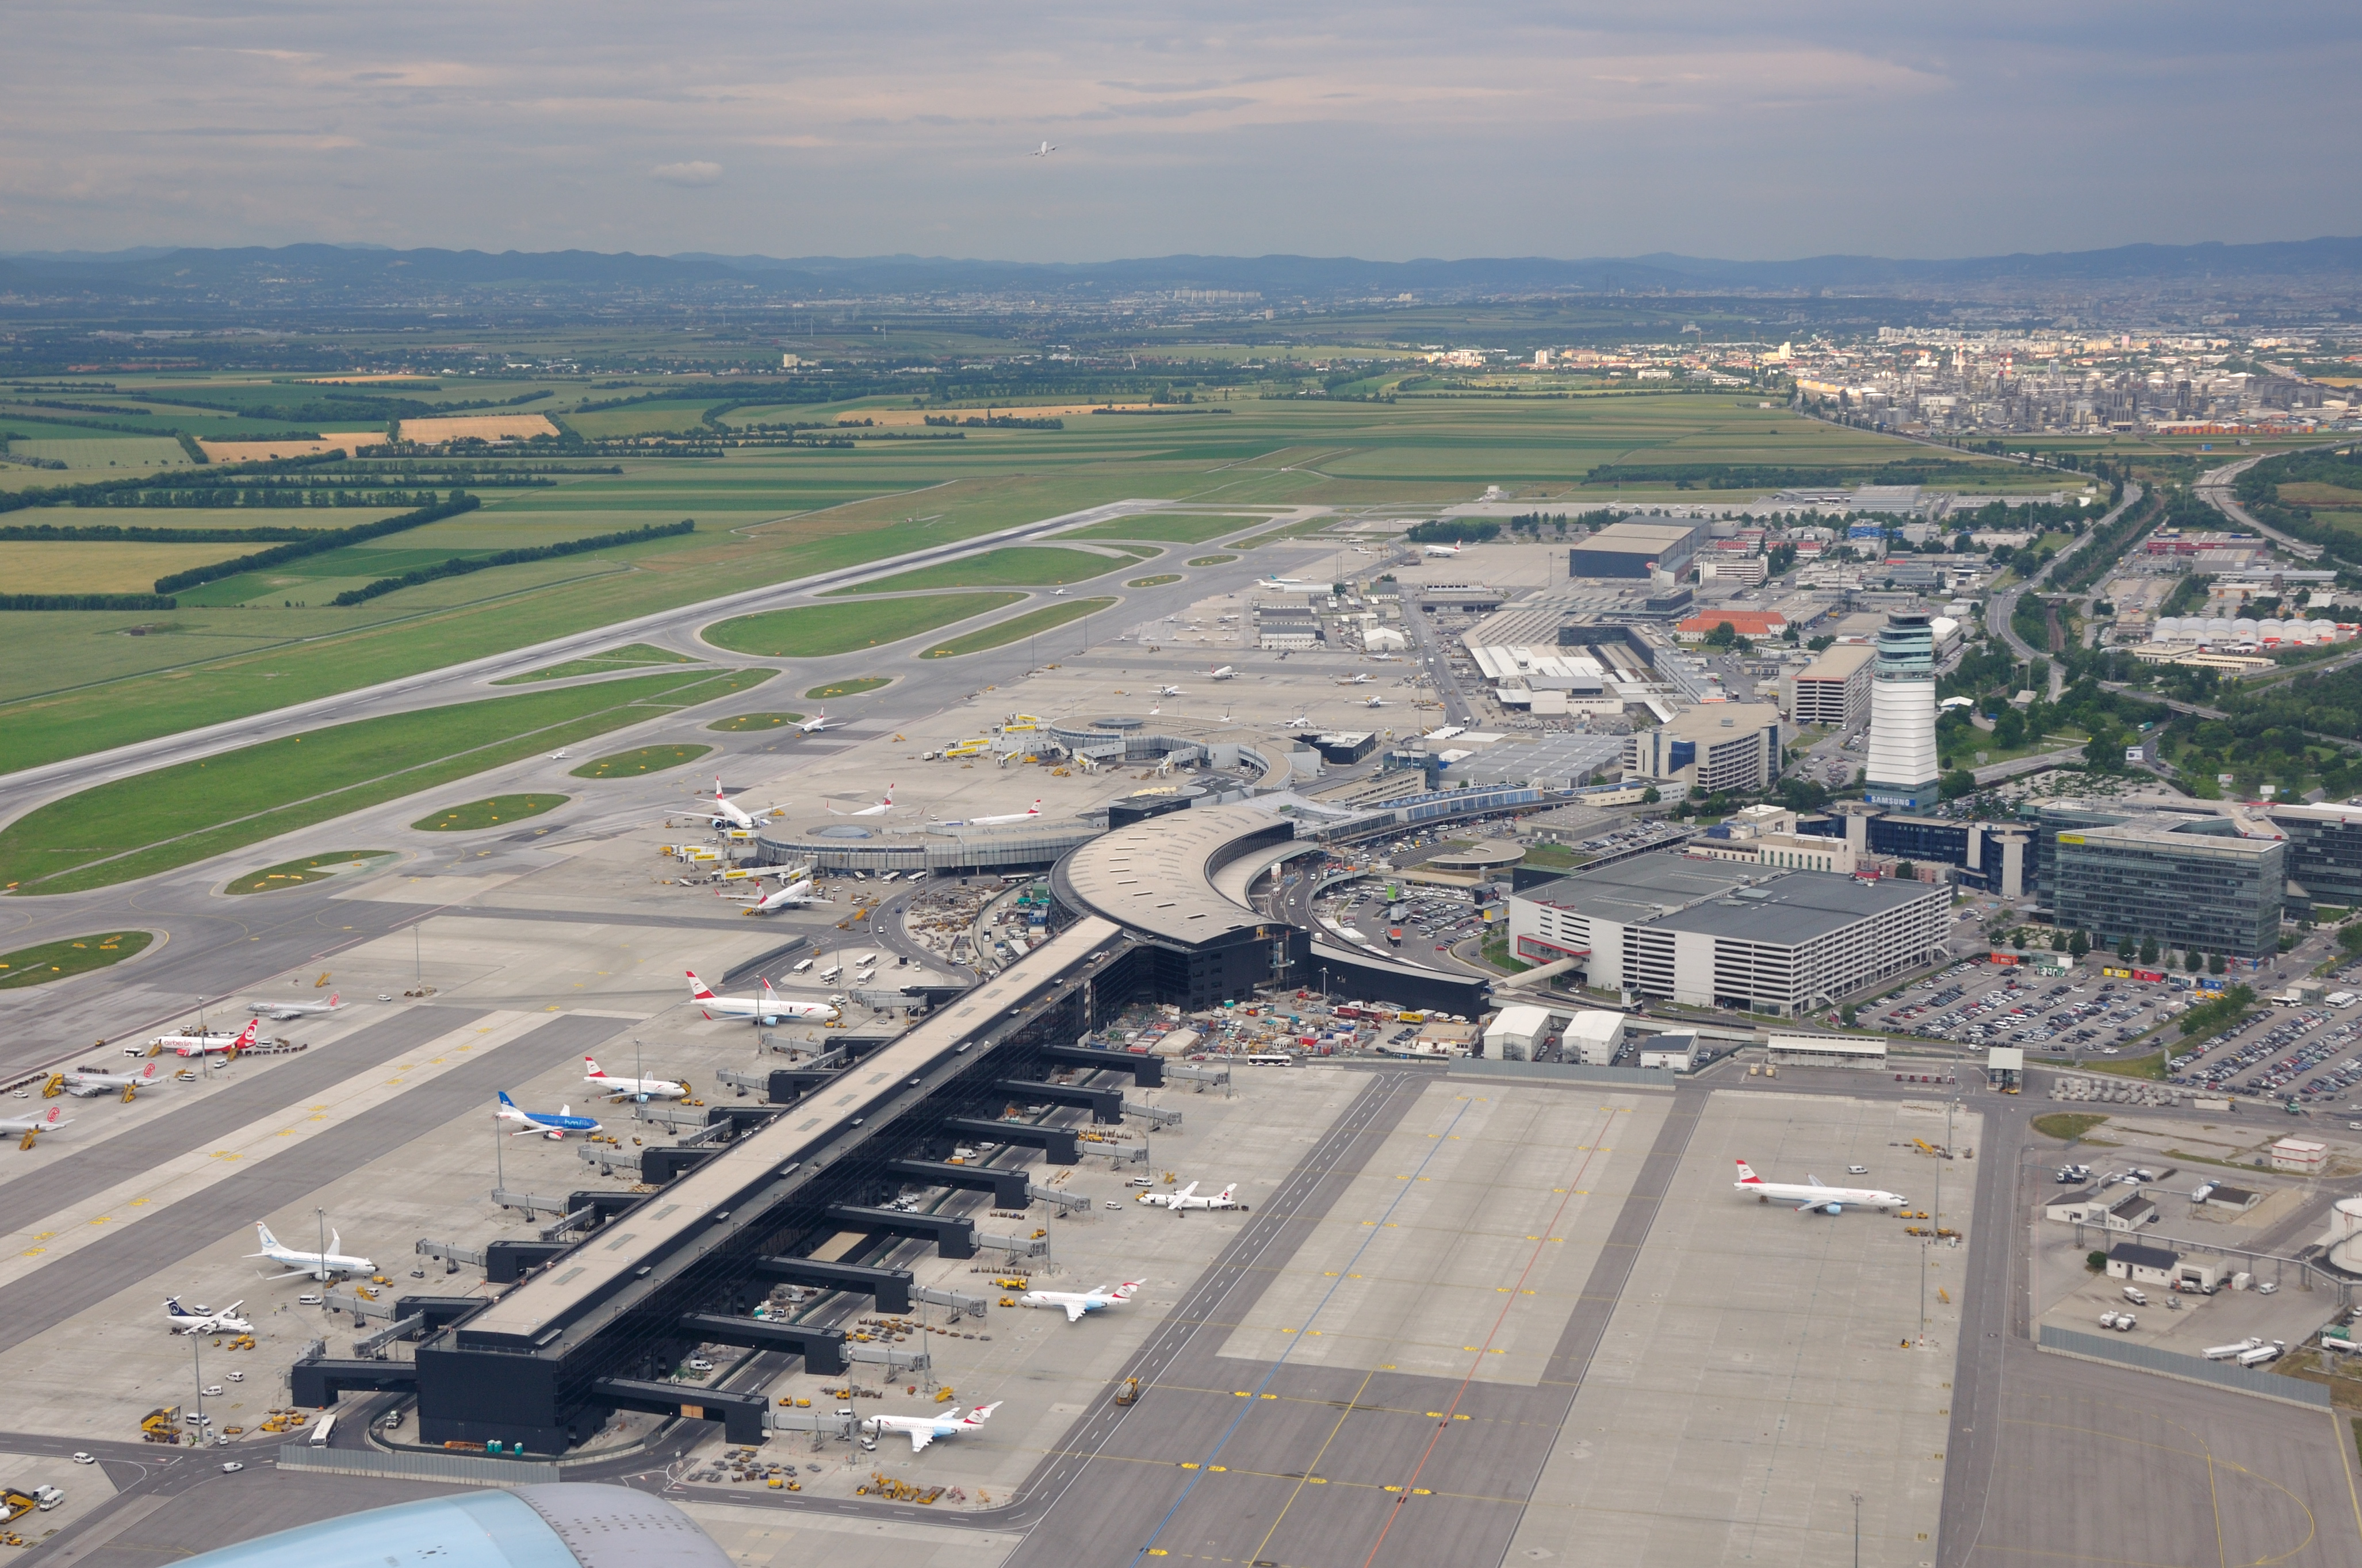
\includegraphics[width=0.7\textwidth]{airport_vienna.jpg}
\footnotesize{Source: Wikipedia}
\end{center}
\end{figure}

\begin{description}
\item[\color{kdedarker} Bratislava] (BTS, 2 mil.) -- 130 km from Brno, 7 airlines serve
regular flights to over 30 destinations, there is a hub of Ryanair
(cheap flights to many European cities). There is no direct connection
between the airport and Brno. Trains (\euro{7}, 1.5 hour) and buses
(\euro{9}, 2 hours) go to Brno from the city center every hour.
\item[\color{kdedarker} Brno] (BRQ, 0.5 mil. passengers transported a year) -- 
connections to London-Stansted (Ryanair), London-Luton (Wizz Air),
Alicante and Bergamo, Italy (Ryanair).
\item[\color{kdedarker} Prague] (PRG, 13 mil.) -- 210 km from Brno, 50 airlines serve flights to over 120 destinations. Student Agency buses go from the airport to Brno every hour (3 hours, CZK\,250/\euro{10}).
\item[\color{kdedarker} Vienna] (VIE, 18 mil.) -- 135 km from Brno, about 70 airlines serve flights to many destinations all over the world. Student Agency buses go from the airport to Brno every other hour
(2.5 hours, CZK\,310/\euro{13}).
\end{description}

\subsubsection*{By Train}
Vienna has good train connections to several European cities and train is the fastest and most convenient
means of transportation between big cities in the region. All trains arrive and depart at the main train
station (Wien Hauptbahnhof).

\begin{description}
\item[\color{kdedarker} Berlin] -- from Berlin Hauptbahnhofm, several trains a day, 7.5~hours, \euro{39}
\item[\color{kdedarker} Bratislava] -- from Bratislava Hlavná Stanica, hourly, 1~hour, \euro{7}
\item[\color{kdedarker} Budapest] -- from Budapest-Keleti, several trains a day, 5~hours, \euro{19}
\item[\color{kdedarker} Prague] -- from Prague Main Station, hourly, 2.5~hours, \euro{13}
\item[\color{kdedarker} Vienna] -- from Vienna Meidling and Brno, every other hour, 2~hours, \euro{13}
\item[\color{kdedarker} Warsaw] -- from Warszawa Centralna, several times a day, 7~hours, \euro{29}
\end{description}

\subsubsection*{By Bus}
Long-distance bus lines to Vienna are operated by the following companies: Flixbus, Eurolines, StudentAgency (from/to Czech Republic),
Orangeways (from/to Hungary), Polskibus (from/to Poland). If booked in advance, these can offer a cheap alternative to trains or flights.

\subsubsection*{By Car}
Vienna is well-connected to other cities by highways. You can get easily to neighboring countries by car.
Travel time examples:

\begin{description}
\item[\color{kdedarker} Berlin] -- 640 km, 6.75 hours
\item[\color{kdedarker} Budapest] -- 243 km, 2.5 hours
\item[\color{kdedarker} Bratislava] -- 80 km, 1 hour
\item[\color{kdedarker} Prague] -- 300 km, 3.5 hours
\item[\color{kdedarker} Brno] -- 134 km, 1.75 hours
\item[\color{kdedarker} Ljubljana] -- 384 km, 3.75 hours
\item[\color{kdedarker} Zagreb] -- 373 km, 4 hours
\end{description}

Parking near the venue and in most inner districts is not free and only possible for short term. We recommend to park either at your accomodation or in a Park \& Ride garage (Cost: 17 \euro for one week).

\subsubsection*{How to get around}
Brno has an efficient public transport which consists of trams, trolley buses, and buses. The main hub is the main railway station. Bus terminals (\mbox{Zvonařka} and
Hotel Grand) lie nearby. The easiest way to get to the venue is to take the tram \#{1}
to Semilasso.

Public transport tickets: CZK\,25 (\euro{1})/60min.

Getting from and to the airport: The bus \#{76} (\#{89} in the night) goes between
the main railway station and the airport. The journey takes 20 minutes. Taxis are
available as well.

\cleardoublepage

\section*{SWAG}
\addcontentsline{toc}{section}{SWAG}
We have promotional goods done quite often and have quality and reliable suppliers for swag. Pricing
examples:

\begin{itemize}
\item A~t-shirt with a big logo/picture -- CZK\,87 (\euro{3.55}) if we order 300 t-shirts.
\item Buttons with a logo -- the normal price is CZK\,750 (\euro{30.61}) for 100 pins. If we order for example 
1,000 pins the total price will be CZK\,7,500 (\euro{306}, we may be eligible for a quantity
discount).
\item Stickers -- CZK\,49 (\euro{2}) for an A4 sheet of quality stickers.
\end{itemize}

\cleardoublepage

\section*{The Venue}
\addcontentsline{toc}{section}{The Venue}

There are several venues in Brno where Akademy could take place. The preferred venue is on Faculty of Information Technology of Brno Technical University (FIT BUT). Due to an unexpected reconstruction works scheduled during the summer, the faculty can only offer date from 5th to 12th September. The faculty has offered to sponsor Akademy by offering 50\% discount from the rent.

We are currently looking into other possible venues, especially Faculty of Informatics of Masaryk University (FI MU).

\section*{Neues EI}
\addcontentsline{toc}{subsection}{Neues EI}

\begin{wrapfigure}{r}{0.5\textwidth}
\vspace{-22pt}
\begin{center}
% \includegraphics[width=0.5\textwidth]{fitvut2.jpg}
\end{center}
\vspace{-16pt}
\end{wrapfigure}
The \mbox{Faculty} of Information Technology at
the Brno University of \mbox{Technology} building used to be a \mbox{Cartesian} monastery founded in the 14\textsuperscript{th}
century. Recently, it was renovated and now features a beautiful combination of historical and modern
architecture. It is located in a calm neighbourhood of Brno within 25 minutes of the city center by tram.
There are several larger lecture rooms in two buildings. The building (D), which we propose for the keynote and main talks, has three lecture rooms:

\begin{description}
\item[\color{kdedarker} D105] -- 300 seats, the most representative room where graduation ceremonies take place.
\item[\color{kdedarker} D0206] -- 154 seats, a lecture room which is located underneath D105.
\item[\color{kdedarker} D0207] -- 90 seats, a lecture room which is located next to D0206.
\end{description}

\begin{center}
% \includegraphics[width=0.5\textwidth]{fitvut3.jpg}
\end{center}

\subsection*{Equipment}
\addcontentsline{toc}{subsubsection}{Equipment}
All lecture \& seminar rooms are equipped with:
\begin{itemize}
	\item a projector,
	\item a cable to connect a laptop to the projector,
	\item audio (hands-free microphones),
	\item video and audio recording,
	\item wifi connection (encrypted, guest accounts would need to be organized)
\end{itemize}

\begin{figure}[ht]
\centering
% \subfloat{\includegraphics[width=0.49\textwidth]{fitvut1.jpg}}\hfill
% \subfloat{\includegraphics[width=0.49\textwidth]{fitvut4.jpg}}
\end{figure}

The entire building is covered by a wireless network.

\newpage

\subsection*{Catering}
\addcontentsline{toc}{subsubsection}{Catering}
There are several options for Akademy attendants to get meals and refershment in the campus:

\begin{description}
\item[\color{kdedarker} University Cafeteria] -- can provide regular meals and drinks for lunch. It can serve a larger number of people.
\item[\color{kdedarker} Restaurant Old Brewery] -- is in the same building as the university cafeteria, provides daily meals during lunch time and usual offering of meals and drinks. It may provide meals without previous order.
\item[\color{kdedarker} Café Ventana] -- is situated in the same building. The café sells hot and cold beverages, cakes, and snacks.
\item[\color{kdedarker} Catering On Site] -- basic catering (mineral water, hot
beverages, snacks) could be provided on site, so that attendants can get refreshment
between talks. There are many other restaurants and pubs within a few minutes walk
from the venue, most of them with free wifi access.
\end{description}


\section*{Freihaus}
\addcontentsline{toc}{subsection}{FI MU}


There faculty has three big lecture rooms:
\begin{description}
\item[\color{kdedarker} D1] -- 248 seats
\item[\color{kdedarker} D2] -- 122 seats
\item[\color{kdedarker} D3] -- 179 seats
\end{description}

There are also many smaller lecture rooms and class rooms that could be used for BoF sessions.

\subsection*{Equipment}
\addcontentsline{toc}{subsubsection}{Equipment}
All lecture \& seminar rooms are equipped with:
\begin{itemize}
\item a projector,
\item a cable to connect a laptop to the projector,
\item audio (hands-free microphones),
\item video and audio recording,
\item wifi connection (encrypted, guest accounts would need to be organized)
\end{itemize}

The entire building is covered by a wireless network.

\begin{figure}[ht]
\centering
% \subfloat{\includegraphics[width=0.49\textwidth]{fimu1.jpg}}\hfill
% \subfloat{\includegraphics[width=0.49\textwidth]{fimu2.jpg}}
\end{figure}



\subsection*{Catering}
\addcontentsline{toc}{subsubsection}{Equipment}
There is no cafeteria in the building, but there are several restaurants around the faculty:

\begin{description}
\item[\color{kdedarker} Al Capone] -- italian restaurant, offers several vegatarian meals -- \sloppy \mbox{\url{www.pizzaalcapone.cz}}
\item[\color{kdedarker} Magistr] -- a microbrewery with restarurant -- \url{www.pivovarmagistr.cz}
\item[\color{kdedarker} AURA restaurant] -- restaurant, cafe, bar -- \url{www.campea.cz}
\item[\color{kdedarker} Catering On Site] -- basic catering (mineral water, hot
beverages, snacks) could be provided on site, so that attendants can get refreshment
between talks
\end{description}


\newpage

\section*{Social Events}
\addcontentsline{toc}{section}{Social Events}

\begin{wrapfigure}{r}{0.3\textwidth}
\vspace{-22pt}
\begin{center}
% \includegraphics[width=0.3\textwidth]{fleda.jpg}
\footnotesize{Source: Michal Sänger - BY-CN-SA}
\vspace{-20pt}
\end{center}
\end{wrapfigure}

Brno offers good venues to organize conference parties. Some of them are
really close to the proposed conference venue. Here are some we propose
because we've already organized social events there and have good
experience with them:

\begin{description}
\item[\color{kdedarker} Fléda] -- a large venue for concerts and other events which is located
30 minutes walk from the conference venue. It has capacity up to 800 people.
The rent for one night is CZK\,31,700 (\euro{1,230}) and can provide discount
on catering. Fléda website: \url{http://www.fleda.cz}
\item[\color{kdedarker} Semilasso] -- venue for concerts and other events which is
just a few hundred meters from the conference venue. The main hall
has capacity 700 people, the garden 300 people. The rent for one night
is CZK\,35,000 (\euro{1,355}). The club is also suitable for concerts,
both outside and inside. The club's website:
\url{http://www.semilasso.cz/}
\item[\color{kdedarker} Brewery Brno] -- a large restaurant located on the premises of
Brno's brewery. The capacity of the main hall is at least 300 people.
It has a dance floor and a DJ can be arranged. A~rent for one night is
CZK\,90,000 (\euro{3,673}). The rent is free if you order catering. The
restaurant's website:
\url{http://www.pivovarskabrno.cz/}
\end{description}

\cleardoublepage

\section*{Accomodation}
\addcontentsline{toc}{section}{Accomodation}
We'd like to provide several price levels of accommodation to suit to all conference attendants:

\subsection*{Low Cost}
\addcontentsline{toc}{subsection}{Low Cost}
\begin{itemize}
\item \emph{Student Dormitories} of the Mendel University in Brno -- 
are the cheapest accommodation option. They can provide a
large number of rooms. The current price is CZK\,600 (\euro{23.3}) for a
double-bed room and CZK\,400 (\euro{15.5}) for single-bed room. Breakfast is additional
CZK\,110 (\euro{4.3}). The dormitories have facilities
such as a student cafeteria, pizzeria, sport facilities, and even a
cinema. The campus is just 3~bus stops away from the venue and the bus
53 takes you almost from door to door. If you feel like stretching your
legs a bit the pleasent walk will take you about 15 -- 20 minutes. A~tram
takes you to the old town in about 20 minutes.
\end{itemize}

\begin{figure}[ht]
\begin{center}
% \includegraphics[width=0.6\textwidth]{tauferky.jpg}
\end{center}
\end{figure}

\subsection*{Mid-Range}
\addcontentsline{toc}{subsection}{Mid-Range}
\begin{itemize}
\item \emph{Hotel Avanti} $\star\star\star\star{}$ -- is another mid-range option we recommend. One
double bed room is CZK\,1,690 (\euro{69}) for one person and CZK\,1,840
(\euro{75} for two persons). The hotel also offers more expensive
options up to a President suite for CZK\,4,890 (\euro{200}). It might be possible
to arrange a discount for Akademy attendees. The hotel is 15
minutes (tram), 25 minutes (walking) from the conference venue. And it's
just 12 minutes by tram to get to the city center. The hotel's website:
\url{http://www.brno-hotel-avanti.eu/}
\end{itemize}


\begin{figure}[ht]
\begin{center}
% \includegraphics[width=0.7\textwidth]{avanti.jpg}
\end{center}
\end{figure}

\subsection*{High-end}
\addcontentsline{toc}{subsection}{High-end}
\begin{itemize}
\item \emph{Barceló Brno Palace} $\star\star\star\star{}$+ -- the newest and one of the most luxurious hotels in Brno
has airy interior with Spanish-style design and a very good restaurant. It satisfies the highest
standards. Rooms start at \euro{137}. It takes 10 minutes by car (20 minutes by tram) to get from
the hotel to the venue, the city center is just a few minutes of walking away. The hotel's web-
site: \sloppy \url{http://www.barcelobrnopalace.com/BarceloHotels/en\_GB/hotels/Czech-Republic/Brno/
hotel-barcelo-brno-palace/general-description.aspx}
\end{itemize}

\begin{figure}[ht]
\begin{center}
% \includegraphics[width=0.7\textwidth]{barcelo.jpg}
\end{center}
\end{figure}

\cleardoublepage

\section*{Contact}
\addcontentsline{toc}{section}{Contact}
\Author

\end{document}
